% Options for packages loaded elsewhere
\PassOptionsToPackage{unicode}{hyperref}
\PassOptionsToPackage{hyphens}{url}
\PassOptionsToPackage{dvipsnames,svgnames*,x11names*}{xcolor}
%
\documentclass[
  12pt, krantz2,
]{krantz}

\usepackage{amsmath,amssymb}
\usepackage{lmodern}
\usepackage{iftex}
\ifPDFTeX
  \usepackage[T1]{fontenc}
  \usepackage[utf8]{inputenc}
  \usepackage{textcomp} % provide euro and other symbols
\else % if luatex or xetex
  \usepackage{unicode-math}
  \defaultfontfeatures{Scale=MatchLowercase}
  \defaultfontfeatures[\rmfamily]{Ligatures=TeX,Scale=1}
  % \usepackage{fontspec}
  \setmainfont{Comic Sans MS}
  \setmonofont[Scale=0.85]{Inconsolata}
\fi
% Use upquote if available, for straight quotes in verbatim environments
\IfFileExists{upquote.sty}{\usepackage{upquote}}{}
\IfFileExists{microtype.sty}{% use microtype if available
  \usepackage[]{microtype}
  \UseMicrotypeSet[protrusion]{basicmath} % disable protrusion for tt fonts
}{}
\makeatletter
\@ifundefined{KOMAClassName}{% if non-KOMA class
  \IfFileExists{parskip.sty}{%
    \usepackage{parskip}
  }{% else
    \setlength{\parindent}{0pt}
    \setlength{\parskip}{6pt plus 2pt minus 1pt}}
}{% if KOMA class
  \KOMAoptions{parskip=half}}
\makeatother
\usepackage{xcolor}
\IfFileExists{xurl.sty}{\usepackage{xurl}}{} % add URL line breaks if available
\IfFileExists{bookmark.sty}{\usepackage{bookmark}}{\usepackage{hyperref}}
\hypersetup{
  pdftitle={Data Science for Kids},
  pdfauthor={Haim Bar, HaiYing Wang, and Jun Yan},
  colorlinks=true,
  linkcolor={Maroon},
  filecolor={Maroon},
  citecolor={Blue},
  urlcolor={Blue},
  pdfcreator={LaTeX via pandoc}}
\urlstyle{same} % disable monospaced font for URLs
\usepackage{color}
\usepackage{fancyvrb}
\newcommand{\VerbBar}{|}
\newcommand{\VERB}{\Verb[commandchars=\\\{\}]}
\DefineVerbatimEnvironment{Highlighting}{Verbatim}{commandchars=\\\{\}}
% Add ',fontsize=\small' for more characters per line
\usepackage{framed}
\definecolor{shadecolor}{RGB}{248,248,248}
\newenvironment{Shaded}{\begin{snugshade}}{\end{snugshade}}
\newcommand{\AlertTok}[1]{\textcolor[rgb]{0.33,0.33,0.33}{#1}}
\newcommand{\AnnotationTok}[1]{\textcolor[rgb]{0.37,0.37,0.37}{\textbf{\textit{#1}}}}
\newcommand{\AttributeTok}[1]{\textcolor[rgb]{0.61,0.61,0.61}{#1}}
\newcommand{\BaseNTok}[1]{\textcolor[rgb]{0.06,0.06,0.06}{#1}}
\newcommand{\BuiltInTok}[1]{#1}
\newcommand{\CharTok}[1]{\textcolor[rgb]{0.5,0.5,0.5}{#1}}
\newcommand{\CommentTok}[1]{\textcolor[rgb]{0.37,0.37,0.37}{\textit{#1}}}
\newcommand{\CommentVarTok}[1]{\textcolor[rgb]{0.37,0.37,0.37}{\textbf{\textit{#1}}}}
\newcommand{\ConstantTok}[1]{\textcolor[rgb]{0,0,0}{#1}}
\newcommand{\ControlFlowTok}[1]{\textcolor[rgb]{0.27,0.27,0.27}{\textbf{#1}}}
\newcommand{\DataTypeTok}[1]{\textcolor[rgb]{0.27,0.27,0.27}{#1}}
\newcommand{\DecValTok}[1]{\textcolor[rgb]{0.06,0.06,0.06}{#1}}
\newcommand{\DocumentationTok}[1]{\textcolor[rgb]{0.37,0.37,0.37}{\textbf{\textit{#1}}}}
\newcommand{\ErrorTok}[1]{\textcolor[rgb]{0.14,0.14,0.14}{\textbf{#1}}}
\newcommand{\ExtensionTok}[1]{#1}
\newcommand{\FloatTok}[1]{\textcolor[rgb]{0.06,0.06,0.06}{#1}}
\newcommand{\FunctionTok}[1]{\textcolor[rgb]{0,0,0}{#1}}
\newcommand{\ImportTok}[1]{#1}
\newcommand{\InformationTok}[1]{\textcolor[rgb]{0.37,0.37,0.37}{\textbf{\textit{#1}}}}
\newcommand{\KeywordTok}[1]{\textcolor[rgb]{0.27,0.27,0.27}{\textbf{#1}}}
\newcommand{\NormalTok}[1]{#1}
\newcommand{\OperatorTok}[1]{\textcolor[rgb]{0.43,0.43,0.43}{\textbf{#1}}}
\newcommand{\OtherTok}[1]{\textcolor[rgb]{0.37,0.37,0.37}{#1}}
\newcommand{\PreprocessorTok}[1]{\textcolor[rgb]{0.37,0.37,0.37}{\textit{#1}}}
\newcommand{\RegionMarkerTok}[1]{#1}
\newcommand{\SpecialCharTok}[1]{\textcolor[rgb]{0,0,0}{#1}}
\newcommand{\SpecialStringTok}[1]{\textcolor[rgb]{0.5,0.5,0.5}{#1}}
\newcommand{\StringTok}[1]{\textcolor[rgb]{0.5,0.5,0.5}{#1}}
\newcommand{\VariableTok}[1]{\textcolor[rgb]{0,0,0}{#1}}
\newcommand{\VerbatimStringTok}[1]{\textcolor[rgb]{0.5,0.5,0.5}{#1}}
\newcommand{\WarningTok}[1]{\textcolor[rgb]{0.37,0.37,0.37}{\textbf{\textit{#1}}}}
\usepackage{longtable,booktabs,array}
\usepackage{calc} % for calculating minipage widths
% Correct order of tables after \paragraph or \subparagraph
\usepackage{etoolbox}
\makeatletter
\patchcmd\longtable{\par}{\if@noskipsec\mbox{}\fi\par}{}{}
\makeatother
% Allow footnotes in longtable head/foot
\IfFileExists{footnotehyper.sty}{\usepackage{footnotehyper}}{\usepackage{footnote}}
\makesavenoteenv{longtable}
\usepackage{graphicx}
\makeatletter
\def\maxwidth{\ifdim\Gin@nat@width>\linewidth\linewidth\else\Gin@nat@width\fi}
\def\maxheight{\ifdim\Gin@nat@height>\textheight\textheight\else\Gin@nat@height\fi}
\makeatother
% Scale images if necessary, so that they will not overflow the page
% margins by default, and it is still possible to overwrite the defaults
% using explicit options in \includegraphics[width, height, ...]{}
\setkeys{Gin}{width=\maxwidth,height=\maxheight,keepaspectratio}
% Set default figure placement to htbp
\makeatletter
\def\fps@figure{htbp}
\makeatother
\setlength{\emergencystretch}{3em} % prevent overfull lines
\providecommand{\tightlist}{%
  \setlength{\itemsep}{0pt}\setlength{\parskip}{0pt}}
\setcounter{secnumdepth}{5}
\usepackage{booktabs}
\usepackage{longtable}
\usepackage{bbm}
\usepackage[bf,singlelinecheck=off]{caption}

\usepackage{framed,color}
\definecolor{shadecolor}{RGB}{248,248,248}

\usepackage{float}
\floatplacement{figure}{H}
\floatplacement{table}{H}
\setlength{\textfloatsep}{0.1cm}
\usepackage{array}
\usepackage{multirow}
%\usepackage[table]{xcolor}
\usepackage{wrapfig}
\usepackage{colortbl}
\usepackage{pdflscape}
\usepackage{tabu}
\usepackage{threeparttable}
\usepackage{threeparttablex}
\usepackage[normalem]{ulem}
\usepackage{makecell}
\usepackage{kotex}

% Changed via Rob Hyndman's suggestions
% https://robjhyndman.com/hyndsight/latex-floats/
\setcounter{topnumber}{2}
\setcounter{bottomnumber}{2}
\setcounter{totalnumber}{4}
\renewcommand{\topfraction}{0.85}
\renewcommand{\bottomfraction}{0.85}
\renewcommand{\textfraction}{0.15}
\renewcommand{\floatpagefraction}{0.7}
% Force images to appear after their definition
\usepackage{flafter}

\renewenvironment{quote}{\begin{VF}}{\end{VF}}
\let\oldhref\href
\renewcommand{\href}[2]{#2\footnote{\url{#1}}}

% \makeatletter
% \newenvironment{kframe}{%
% \medskip{}
% \setlength{\fboxsep}{.8em}
%  \def\at@end@of@kframe{}%
%  \ifinner\ifhmode%
%   \def\at@end@of@kframe{\end{minipage}}%
%   \begin{minipage}{\columnwidth}%
%  \fi\fi%
%  \def\FrameCommand##1{\hskip\@totalleftmargin \hskip-\fboxsep
%  \colorbox{shadecolor}{##1}\hskip-\fboxsep
%      % There is no \\@totalrightmargin, so:
%      \hskip-\linewidth \hskip-\@totalleftmargin \hskip\columnwidth}%
%  \MakeFramed {\advance\hsize-\width
%    \@totalleftmargin\z@ \linewidth\hsize
%    \@setminipage}}%
%  {\par\unskip\endMakeFramed%
%  \at@end@of@kframe}
% \makeatother

% \renewenvironment{Shaded}{\begin{kframe}}{\end{kframe}}

\usepackage{makeidx}
\makeindex

\urlstyle{tt}

%% Need to clean up
\newenvironment{rmdblock}[1]
  {\begin{shaded*}
  \begin{itemize}
  \renewcommand{\labelitemi}{
    \raisebox{-.7\height}[0pt][0pt]{
  %    {\setkeys{Gin}{width=3em,keepaspectratio}\includegraphics{images/#1}}
    }
  }
  \item
  }
  {
  \end{itemize}
  \end{shaded*}
  }

\newenvironment{rmdnote}
  {\begin{rmdblock}{note}}
  {\end{rmdblock}}
\newenvironment{rmdcaution}
  {\begin{rmdblock}{caution}}
  {\end{rmdblock}}
\newenvironment{rmdimportant}
  {\begin{rmdblock}{important}}
  {\end{rmdblock}}
\newenvironment{rmdtip}
  {\begin{rmdblock}{tip}}
  {\end{rmdblock}}
\newenvironment{rmdwarning}
  {\begin{rmdblock}{warning}}
  {\end{rmdblock}}
\newenvironment{learncheck}
  {\begin{rmdblock}{warning}}
  {\end{rmdblock}}
\newenvironment{review}
  {\begin{rmdblock}{warning}}
  {\end{rmdblock}}
\newenvironment{announcement}
  {\begin{rmdblock}{warning}}
  {\end{rmdblock}}

% No widow lines
% Copied from https://github.com/hadley/adv-r/blob/master/latex/preamble.tex
\widowpenalty=10000
\clubpenalty=10000

\usepackage{amsthm}
\makeatletter
\def\thm@space@setup{%
  \thm@preskip=8pt plus 2pt minus 4pt
  \thm@postskip=\thm@preskip
}
\makeatother

% \listfiles

%%% the preamble from knitr
\definecolor{fgcolor}{rgb}{0.345, 0.345, 0.345}
\newcommand{\hlnum}[1]{\textcolor[rgb]{0.686,0.059,0.569}{#1}}%
\newcommand{\hlstr}[1]{\textcolor[rgb]{0.192,0.494,0.8}{#1}}%
\newcommand{\hlcom}[1]{\textcolor[rgb]{0.678,0.584,0.686}{\textit{#1}}}%
\newcommand{\hlopt}[1]{\textcolor[rgb]{0,0,0}{#1}}%
\newcommand{\hlstd}[1]{\textcolor[rgb]{0.345,0.345,0.345}{#1}}%
\newcommand{\hlkwa}[1]{\textcolor[rgb]{0.161,0.373,0.58}{\textbf{#1}}}%
\newcommand{\hlkwb}[1]{\textcolor[rgb]{0.69,0.353,0.396}{#1}}%
\newcommand{\hlkwc}[1]{\textcolor[rgb]{0.333,0.667,0.333}{#1}}%
\newcommand{\hlkwd}[1]{\textcolor[rgb]{0.737,0.353,0.396}{\textbf{#1}}}%
\let\hlipl\hlkwb

\usepackage{framed}
\makeatletter
\newenvironment{kframe}{%
 \def\at@end@of@kframe{}%
 \ifinner\ifhmode%
  \def\at@end@of@kframe{\end{minipage}}%
  \begin{minipage}{\columnwidth}%
 \fi\fi%
 \def\FrameCommand##1{\hskip\@totalleftmargin \hskip-\fboxsep
 \colorbox{shadecolor}{##1}\hskip-\fboxsep
     % There is no \\@totalrightmargin, so:
     \hskip-\linewidth \hskip-\@totalleftmargin \hskip\columnwidth}%
 \MakeFramed {\advance\hsize-\width
   \@totalleftmargin\z@ \linewidth\hsize
   \@setminipage}}%
 {\par\unskip\endMakeFramed%
 \at@end@of@kframe}
\makeatother

\definecolor{shadecolor}{rgb}{.97, .97, .97}
\definecolor{messagecolor}{rgb}{0, 0, 0}
\definecolor{warningcolor}{rgb}{1, 0, 1}
\definecolor{errorcolor}{rgb}{1, 0, 0}
\newenvironment{knitrout}{}{} % an empty environment to be redefined in TeX

\usepackage{alltt}
\IfFileExists{upquote.sty}{\usepackage{upquote}}{}
%%% end of the preamble from knitr

% self defined environment and commands
\newcounter{example}% [section]
\newenvironment{example}[1][]{\refstepcounter{example}\par\medskip
   \noindent \textbf{Example~\theexample. (#1)} \rmfamily}{\medskip}
   % \noindent \textbf{Example~\thesection.\theexample. (#1)} \rmfamily}{\medskip}

% \theoremstyle{remark}
% \newtheorem*{remark}{Remark}% [section]


%%%%%%%%%%%%%%%%%%%%%%%%%%%%%%%%%%%%%%%%%%%%%%%%%%%%%%%%%%%%
%% from copulaR
\usepackage{mathtools}% fix amsmath deficiencies
\usepackage{amssymb}% sophisticated mathematical symbols with amstex
\usepackage{amsthm}% theorem environments
\usepackage{thmtools}% for declaring theorems

% Theorems
\newif\ifstarttheorem

% For everything but examples and fallacies
\declaretheoremstyle[%
  spaceabove=0.5em,
  spacebelow=0.5em,
  headfont=\sffamily\bfseries\global\starttheoremtrue,
  notefont=\sffamily\bfseries,
  notebraces={(}{)},
  headpunct={},
  bodyfont=\normalfont,
  postheadspace=\newline,%
  qed=\qedsymbol%
  % => If an example ends with a figure which is pushed to the next page (or
  %    just further than 'here'), the qed symbol is not placed correctly.
  %    => Need to work with \clearpage (*before* the figure) at the final
  %       editing stage
  % Note: A hook of the following form did not provide better results:
  % postfoothook={\vspace{-0.5\baselineskip}\hfill\qedsymbol}% we cannot push it further up (in case example ends with text)
]{mythmstyle}
\declaretheorem[style=mythmstyle, numberwithin=section]{definition}% activate style
\declaretheorem[style=mythmstyle, sibling=definition]{lemma}
\declaretheorem[style=mythmstyle, sibling=definition]{proposition}
\declaretheorem[style=mythmstyle, sibling=definition]{theorem}
\declaretheorem[style=mythmstyle, sibling=definition]{corollary}
\declaretheorem[style=mythmstyle, sibling=definition]{remark}
\declaretheorem[style=mythmstyle, sibling=definition]{algorithm}
\declaretheorem[style=mythmstyle, sibling=definition]{illustration}

% For fallacies
\declaretheorem[style=mythmstyle]{fallacy}% no 'sibling = definition'
%%%%%%%%%%%%%%%%%%%%%%%%%%%%%%%%%%%%%%%%%%%%%%%%%%%%%%%%%%%%

% for commenting
\newcommand{\jy}[1]{\textcolor{blue}{(JY: #1)}}


\frontmatter

% \ifLuaTeX
%   \usepackage{selnolig}  % disable illegal ligatures
% \fi

\usepackage[]{natbib}
\bibliographystyle{apalike}

\title{Stumbling into Data Science}
\author{Haim Bar, HaiYing Wang, and Jun Yan}
\date{\today}

\begin{document}
\maketitle

% you may need to leave a few empty pages before the dedication page (CRC guidelines are that the Table of Contents starts on page v. The title page is page i.)
\cleardoublepage\newpage

\thispagestyle{empty}

\begin{center}
  Haim: To my family ... ...
  

  \bigskip

  HaiYing: To my family ... ...

  \bigskip

  Jun: To Jo, Bo, and Jiafeng, without whom the book would have been finished
  much sooner, but life would be unimaginable.
  
\end{center}


{
\hypersetup{linkcolor=}
\setcounter{tocdepth}{2}
\tableofcontents
}

\hypertarget{notes-for-ourselves}{%
\chapter*{Notes for ourselves}\label{notes-for-ourselves}}


\hypertarget{styles}{%
\section*{Styles}\label{styles}}


Basic template for R Markdown from Wenjie Wang
\href{https://statds.org/template/}{at Stat Data Science Lab} with
\href{https://github.com/statds/dslab-templates/}{source}.

\begin{itemize}
\tightlist
\item
  Keep line width under 80 characters for tidy source view.
\item
  No labeling equations unless references.
\item
  Cross-references labels

  \begin{itemize}
  \tightlist
  \item
    chapters: \texttt{ch:estimation}; Chapter\textasciitilde@ref\{ch:estimation\}
  \item
    equations: \texttt{eq:area}
  \item
    tables: \texttt{tab:simu}
  \item
    figures: \texttt{fig:normhist}
  \end{itemize}
\item
  R chunk lables: include chapter index to avoid unwanted duplicates
\item
  Index when appropriate for key words.
\end{itemize}

\hypertarget{reminders}{%
\section*{Reminders}\label{reminders}}

\begin{itemize}
\tightlist
\item
  Bib entries for R packages are generated by a chunk at the end of this file;
  its output \texttt{packages.bib} are not tracked in the repo.
\item
  The dedication page is controlled by \texttt{latex/before\_body.tex}.
\item
  Keep pdf/html consistent as much as possible (need to learn a lot)
\end{itemize}

\hypertarget{preface}{%
\chapter*{Preface}\label{preface}}


\hypertarget{who-this-book-is-for}{%
\section*{Who this book is for}\label{who-this-book-is-for}}


This book is the product of our efforts to promote data science among
high school students.

Many interesting points \ldots{}

\hypertarget{how-to-read-this-book}{%
\section*{How to read this book}\label{how-to-read-this-book}}


Some chapters can be skipped \ldots{}

\hypertarget{computing-language}{%
\section*{Computing language}\label{computing-language}}


We use R because \ldots{}

\hypertarget{about-the-authors}{%
\section*{About the authors}\label{about-the-authors}}


\textbf{Haim Bar} is an Associate Professor in the Department of Statistics,
University of Connecticut. He does a lof of interesting things \ldots{}

\textbf{HaiYing Wang} is an Associate Professor in the Department of Statistics,
University of Connecticut. He does a lof of interesting things \ldots{}

\textbf{Jun Yan} is a Professor in the Department of Statistics,
University of Connecticut. He does a lof of interesting things \ldots{}

All three authors have been members of the Computer Committee of the Department
for years, during which time the idea of the book emerged.

\hypertarget{prerequisites}{%
\chapter*{Prerequisites}\label{prerequisites}}


We hope the widest accessibility.

To compile this example to PDF, you need XeLaTeX. You are recommended to install
TinyTeX\index{TinyTex} (which includes XeLaTeX): \url{https://yihui.org/tinytex/}.



\mainmatter

\hypertarget{intro}{%
\chapter{Introduction}\label{intro}}

In this class, we will use the \R language, and the RStudio integrated development environment (IDE). Before the first meeting, install the necessary software on your personal computer by executing the following instructions.

\hypertarget{installing-r-and-rstudio}{%
\section{Installing R and Rstudio}\label{installing-r-and-rstudio}}

Go to the website of the Comprehensive R Archive Network (\url{https://cran.r-project.org/}) and download the latest version of R for your operating system (Windows, MacOS, or Linux). As of \today, the latest version is 4.0.4. Follow the installation instructions.

Next, go the Rstudio download website
(\url{https://rstudio.com/products/rstudio/download/}) and get the Desktop version
(open source license). As of \today, the version is 1.4.1106. Follow the
installation instruction. An icon that looks like this:

\includegraphics[width=\textwidth,height=0.025\textheight]{images/RstudioLogo.png}
will be on your computer's desktop. Double-click on this icon to start the R session. The Rstudio IDE will open, and look like this:

\begin{center}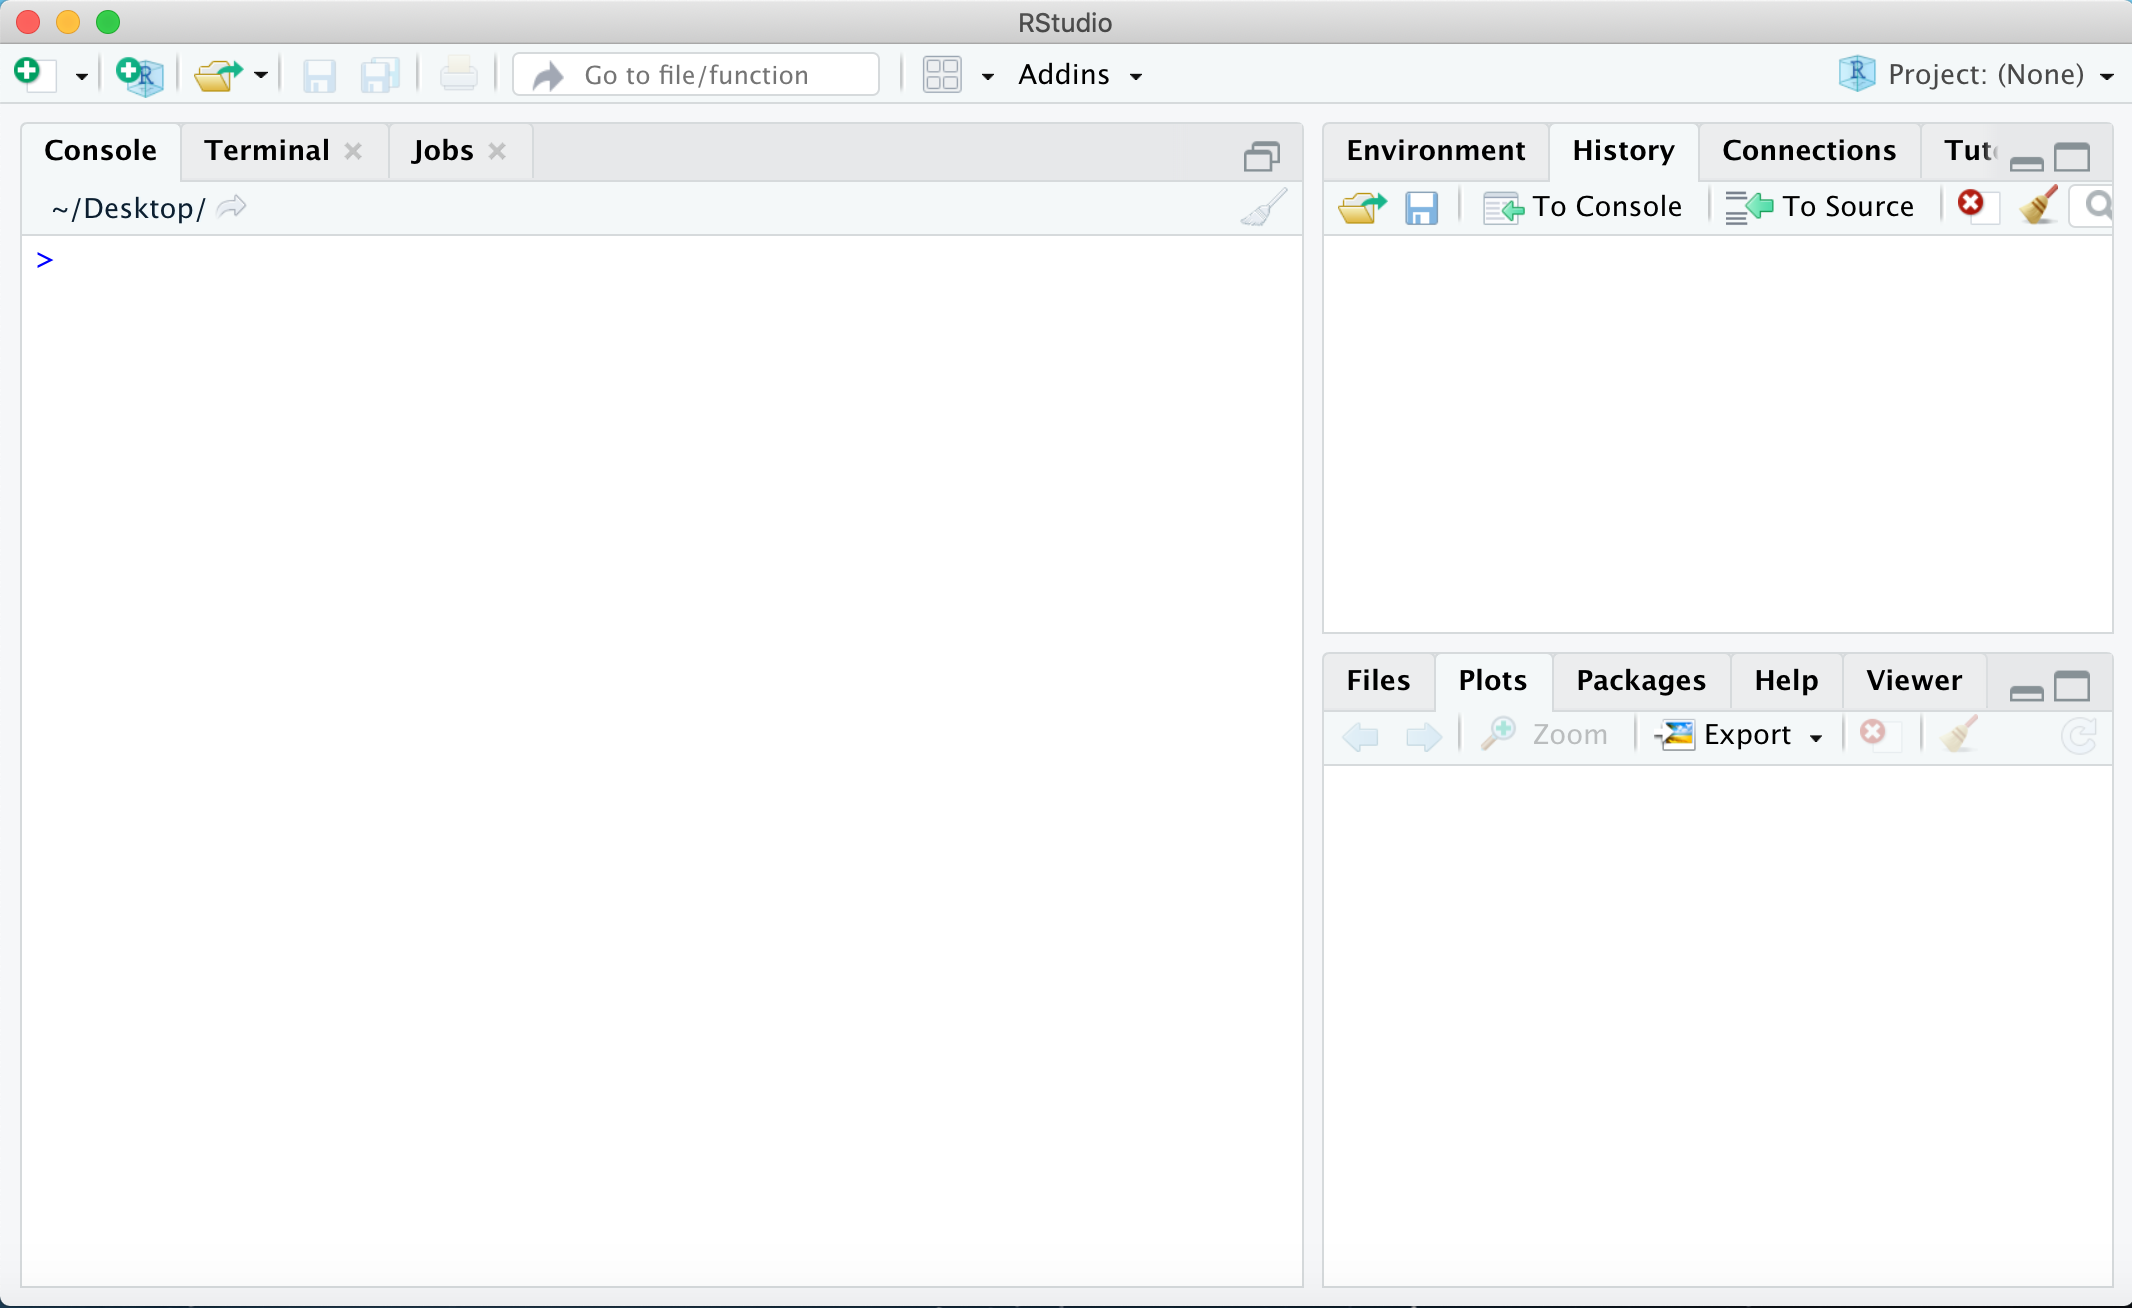
\includegraphics[width=0.7\linewidth]{images/RstudioMain} \end{center}

The left-hand side of the screen contains the Console tab. Notice the \(>\) sign (called the `prompt'). When you see this character, it means that R is ready for the next command. Put the cursor there, and then type

\begin{verbatim}
2 + 2
\end{verbatim}

and hit Enter on the keyboard. You should get the following on the Console:

\begin{verbatim}
[1] 4
\end{verbatim}

Notice the top-right part of the Rstudio window. You should see an `Environment' and a `History' tab. Click on History. Notice that your previous input appears there. Try entering another calculation or command and see that they appear in the session's history. For example, try entering the following

\begin{Shaded}
\begin{Highlighting}[]
\DecValTok{3} \SpecialCharTok{\^{}} \DecValTok{5}
\FunctionTok{date}\NormalTok{()}
\end{Highlighting}
\end{Shaded}

Click on the Environment tab. It should be empty when you start R for the first time. In the Console, type

\begin{Shaded}
\begin{Highlighting}[]
\NormalTok{myFirstVariable }\OtherTok{\textless{}{-}} \FunctionTok{factorial}\NormalTok{(}\DecValTok{5}\NormalTok{)}
\end{Highlighting}
\end{Shaded}

Notice that nothing was printed in the Console, but the Environment tab now contains a table with one row, with `myFirstVariable' appearing in the cell on the left, and its value (120) on the right. Any object appearing in the Environment tab is available to you throughout your R session, and you don't have to recalculate it. For example, you can try the following:

\begin{Shaded}
\begin{Highlighting}[]
\NormalTok{myFirstVariable}\SpecialCharTok{/}\DecValTok{6}
\end{Highlighting}
\end{Shaded}

The Console should now display 20.

The lower-right side of the IDE contains a file browser (the Files tab), information about installed packages (more about it later), and any plot generated during the R session. It also contains a Help tab, to obtain information about built-in functions.

Finally, before we move on to the next section, in the Rstudio top menu, click on File, then on New File, and then on R Script. Alternatively, you can click on little green `+' icon in the top-left part of the IDE. This will split the left side of the Rstudio IDE into two parts -- the lower part will contain the Console, and the top part will contain a tab labeled `Untitled1'. This is were you can enter R code which you will save to a permanent file, and re-use later.
For example, enter the following in the blank space in the Untitled1 tab:

\begin{Shaded}
\begin{Highlighting}[]
\CommentTok{\# This is my first R program}
\FunctionTok{cat}\NormalTok{(}\StringTok{\textquotesingle{}Hello, World!}\SpecialCharTok{\textbackslash{}n}\StringTok{\textquotesingle{}}\NormalTok{)}
\end{Highlighting}
\end{Shaded}

Then, from the main menu in Rstudio, click on File, then on Save, and in the `Save As' box enter FirstProgram.R and click the Save button.
Notice that the tab name is now FirstProgram.R.

In that part of the window, there should now be a small button called Source. Click on it. The program will be executed and the output will be shown in the Console. You can also execute individual lines in the source code. Just put the cursor anywhere in that line, and click on the Run button (which is near the Source button) or click Ctrl+Enter (or Command+Enter on a Mac). 

That's it. In the rest of these notes we will see more features of Rstudio, but you are now ready to start learning programming in R.


\section{Basic Operations in R}
\subsection{Generating random numbers}
In this \hb{course}, much of the learning will be done by using simulated data, so let's start by learning how to generate data. The basic function to generate random data is \code{runif()} which is used to draw random numbers, uniformly between 0 and 1. In the following example we create 10,000 random draws from a uniform distribution, keep these numbers in a variable called simData, and plot a histogram to show the distribution of the data we have generated. The \code{set.seed()} function is used to ensure that every time we run this code, we will get the same set of random numbers. This is called \textit{reproducible code}. 
\begin{knitrout}
\definecolor{shadecolor}{rgb}{0.969, 0.969, 0.969}\color{fgcolor}\begin{kframe}
\begin{alltt}
\hlcom{# Generate 10,000 points from a uniform distribution}
\hlkwd{set.seed}\hlstd{(}\hlnum{210313}\hlstd{)}
\hlstd{n} \hlkwb{<-} \hlnum{10000}
\hlstd{simData} \hlkwb{<-} \hlkwd{runif}\hlstd{(n)}
\hlkwd{hist}\hlstd{(simData)}
\end{alltt}
\end{kframe}\begin{figure}

{\centering 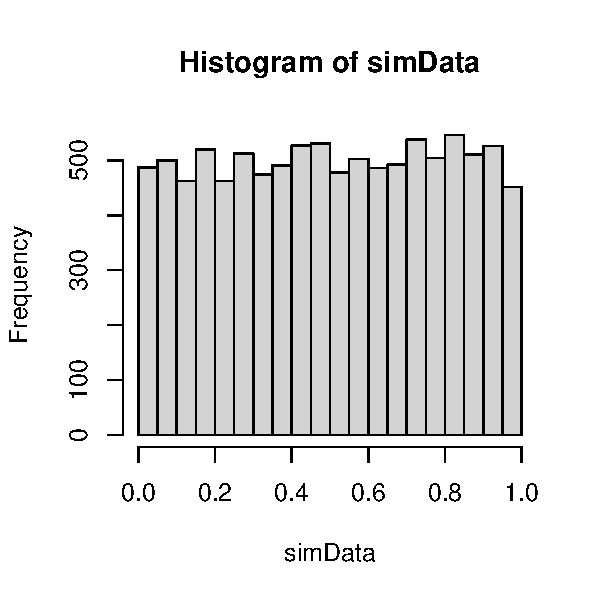
\includegraphics[width=\maxwidth]{figure/intro-runif-1} 

}

\caption[A histogram of 10,000 randomly drawn numbers from a standard uniform distribution]{A histogram of 10,000 randomly drawn numbers from a standard uniform distribution.}\label{fig:intro-runif}
\end{figure}

\end{knitrout}


From the range and the flatness of the histogram we can see that the generated data is indeed uniform on [0,1]. The \code{runif()} function can be used to draw random numbers uniformly on any finite interval. For example, if we want our random numbers to be in the interval [1,5] we will run the following code:

\begin{knitrout}
\definecolor{shadecolor}{rgb}{0.969, 0.969, 0.969}\color{fgcolor}\begin{kframe}
\begin{alltt}
\hlstd{n} \hlkwb{<-} \hlnum{10000}
\hlstd{simData} \hlkwb{<-} \hlkwd{runif}\hlstd{(n,} \hlkwc{min}\hlstd{=}\hlnum{1}\hlstd{,} \hlkwc{max}\hlstd{=}\hlnum{5}\hlstd{)}
\end{alltt}
\end{kframe}
\end{knitrout}

Try it, and draw the histogram as in the previous example. Try it with a fixed seed and verify that you get the same output each time. Then, run the code without a fixed seed and observe that you get a different distribution each time. Since the number of random draws is fairly large, the shape of the histogram will not change much.

From a random draw of a uniform distribution we can generate random numbers from other distributions. For example, we want to simulate (fair) coin flips, and count the number of Heads that we get. Let's say we want to simulate 200 coin tosses. We will draw 200 random numbers from a uniform distribution, and decide that we got Heads in the $i$-th toss if the $i$-the random number is less than 0.5, and Tails otherwise.
Try the following code multiple times (do not use \code{set.seed()}). What do you observe? We will discuss it further in a different \hb{lecture}.
\begin{knitrout}
\definecolor{shadecolor}{rgb}{0.969, 0.969, 0.969}\color{fgcolor}\begin{kframe}
\begin{alltt}
\hlcom{# Simulate 200 coin-flips, using the runif function:}
\hlstd{n.trials} \hlkwb{<-} \hlnum{200}
\hlkwd{cat}\hlstd{(}\hlstr{"Number of Heads is: "}\hlstd{,} \hlkwd{sum}\hlstd{(}\hlkwd{runif}\hlstd{(n.trials)} \hlopt{<} \hlnum{0.5}\hlstd{),} \hlstr{"\textbackslash{}n"}\hlstd{)}
\end{alltt}
\begin{verbatim}
Outout: Number of Heads is:  92
\end{verbatim}
\end{kframe}
\end{knitrout}


A few comments:
\begin{itemize}
\item A comment in \R starts with \#. Any text following the \# sign is considered user-documentation and is not executed by \R.
\item We have used the \code{cat()} function to print (concatenate) text to the console. Fixed text appears in double (or single) quotes, but the content of variables or output from \R functions should not be quoted. The \verb|\n| symbol tells \R to print a newline character at the end. Try to see what happens if you remove it.
\item The expression within the \code{sum()} function produces TRUE/FALSE (Boolean) values. First, we draw n.trials random numbers from a uniform distribution. Then, each one is compared with 0.5. If the value is less than 0.5, the returned value is TRUE. Otherwise, it's FALSE. This demonstrates one of \R's greatest features - allowing to run `vectorized' code. In one line, we generated 200 random numbers and compared each one to 0.5, and as a result, we got 200 Boolean values which we have added together (TRUE counts as 1, and FALSE counts as 0.) So, the result in the sum is the number of Heads in 200 tosses.
\end{itemize}

Statistical inference is based on a mental exercise in which we ask, if we could repeat the same experiment infinitely many times, what would we see? With simulations, we can get a good approximation. For example, the 200 coin-tosses experiment can be repeated, say, 100 times. One way is to use loops, like in the following example:
\begin{knitrout}
\definecolor{shadecolor}{rgb}{0.969, 0.969, 0.969}\color{fgcolor}\begin{kframe}
\begin{alltt}
\hlkwd{set.seed}\hlstd{(}\hlnum{442886}\hlstd{)}
\hlstd{n.trials} \hlkwb{<-} \hlnum{200}  \hlcom{# the number of coin-tosses in each experiment}
\hlstd{reps} \hlkwb{<-} \hlnum{100}  \hlcom{# the number of experiments}
\hlstd{Heads} \hlkwb{<-} \hlkwd{rep}\hlstd{(}\hlnum{0}\hlstd{, reps)}  \hlcom{# A vector to store the results (initialize with 0s)}
\hlkwa{for} \hlstd{(i} \hlkwa{in} \hlnum{1}\hlopt{:}\hlstd{reps) \{}
  \hlstd{Heads[i]} \hlkwb{<-} \hlkwd{sum}\hlstd{((}\hlkwd{runif}\hlstd{(n.trials)} \hlopt{<} \hlnum{0.5}\hlstd{))}
\hlstd{\}}
\hlkwd{hist}\hlstd{(Heads,} \hlkwc{breaks}\hlstd{=}\hlnum{20}\hlstd{)}
\end{alltt}
\end{kframe}\begin{figure}

{\centering 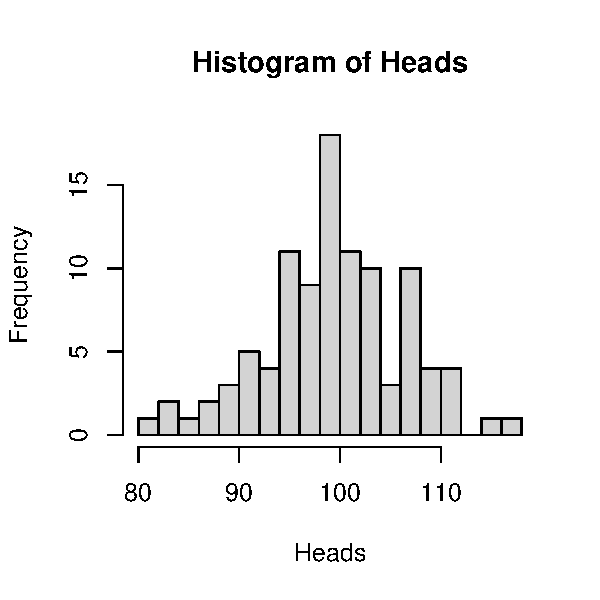
\includegraphics[width=\maxwidth]{figure/intro-heads2-1} 

}

\caption[A histogram of 100 experiments, from each we get the total number of Heads in 200 fair coin tosses]{A histogram of 100 experiments, from each we get the total number of Heads in 200 fair coin tosses.}\label{fig:intro-heads2}
\end{figure}

\end{knitrout}


We've used a \code{for()} loop, with an index variable called \texttt{i} which runs from 1 to 100. In each iteration we simulated n.trials=200 coin tosses, as before. The result from each iteration is stored in the $i$-th position in the vector we called Heads.

Using the uniform distribution, we have created a random draw from a different distribution, called the `binomial'. The mathematical notation is $Bin(N, p)$ where $N$ is the number of trials such that in each trial there can be exactly two outcomes (e.g., coin tosses), and $p$ is the probability of the first possible outcome (e.g., Head), and $1-p$ is the probability of the second possible outcome (e.g., Tail).
\R has a built-in function to generate random numbers from many different distributions, so the code above can be replaced by the following, which uses the \code{rbinom()} function:
\begin{knitrout}
\definecolor{shadecolor}{rgb}{0.969, 0.969, 0.969}\color{fgcolor}\begin{kframe}
\begin{alltt}
\hlkwd{set.seed}\hlstd{(}\hlnum{442886}\hlstd{)}
\hlstd{reps} \hlkwb{<-} \hlnum{100}
\hlstd{n.trials} \hlkwb{<-} \hlnum{200}
\hlstd{Heads} \hlkwb{<-} \hlkwd{rbinom}\hlstd{(reps, n.trials,} \hlnum{0.5}\hlstd{)}
\hlkwd{hist}\hlstd{(Heads,} \hlkwc{breaks}\hlstd{=}\hlnum{20}\hlstd{)}
\end{alltt}
\end{kframe}\begin{figure}

{\centering 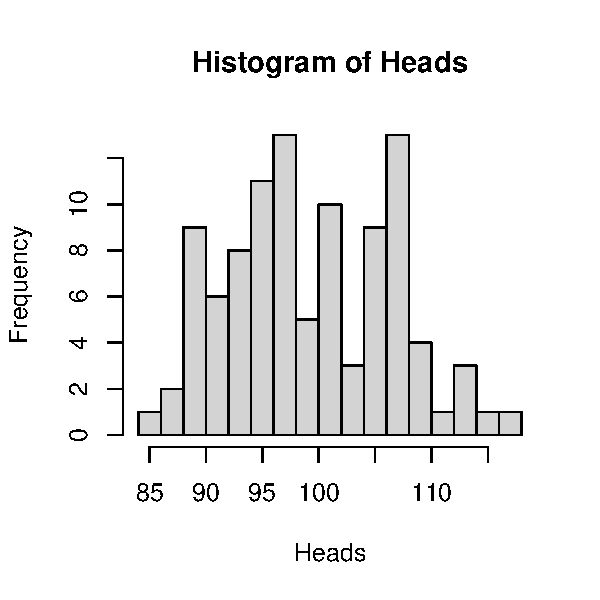
\includegraphics[width=\maxwidth]{figure/intro-binomial-1} 

}

\caption[A histogram of 100 binomial experiments, using rbinom() to simulate 200 fair coin tosses in each experiment]{A histogram of 100 binomial experiments, using rbinom() to simulate 200 fair coin tosses in each experiment.}\label{fig:intro-binomial}
\end{figure}

\end{knitrout}


Exercises:
\begin{enumerate}
\item Change the number of simulated coin-toss datasets (\texttt{reps}) to 1,000 and rerun the code. Then change it to 10,000 and run it again. What do you notice?
\item Change the probability of Heads to 0.2 and run the code again. Then, change it to 0.8. What do you observe?
\item Try other values of the number of trials and the probability of Heads.
\end{enumerate}




\subsection{Summary statistics}
Let's generate some data:
\input{Rnw/intro-rexp1}

We will introduce some statistical functions to summarize data. The most commonly used one is the mean (a.k.a. the average), $\overline{x}$:\\
$$\overline{x}=\frac{x_1+\ldots+x_n}{n}\,.$$
Other ways to estimate some sort of `central tendency' of a distribution are:
 (i) the trimmed mean, which is similar to the mean, except that the smallest and largest $p\cdot 100\%$  of the values are excluded from the computation. For example, if we take $p=0.1$ with the simulated data, only 800 data points are used in the calculation of the trimmed mean; (ii) The median is a number, $x_{0.5}$, such that half the data points are greater than $x_{0.5}$ and half are less than or equal to $x_{0.5}$. 

Try the following:
\input{Rnw/intro-rexp2}

The distribution of $x$ is shown below as a \textit{box-and-whisker plot} (or simply, boxplot). This is a very simple representation of numeric data, which is constructed by summarizing the data using a few numeric characteristics. The boxplot below is drawn horizontally, and the vertical grey line inside the box is the median. Similar to the median, we find the first quartile -- a point $x_{25}$ such that 25\% of the values are less than $x_{25}$ and 75\% are greater than $x_{25}$; and the third quartile -- a point $x_{75}$ such that 75\% of the values are less than $x_{75}$ and 25\% are greater than $x_{75}$. The first and third quartiles are the vertical edges of the box, also called the lower and upper hinges. So, the box represents 50\% of the data. The range between the first and third quartiles is called the \textit{Inter-Quartile Range}, or IQR.
The `whiskers', which are the dashed grey lines, are constructed by adding 1.5$\cdot$IQR to each side of the box. If the result is smaller than the minimum value (or greater than the maximum), then the whisker only extends to the minimum (maximum). Points within the range between the two whiskers are not plotted individually, since their distribution is summarized succinctly by the box-and-whiskers plot. Points outside the range between the two whiskers are considered `outliers', or extreme values, and are shown explicitly. 


A boxplot does not include the mean, or the trimmed mean, but we have added them here as a red circle and brown diamond, respectively, in order to show that they are different than the mean. The mean is smaller in this case, because the distribution is skewed to the left -- there are many more data points in the range closer to zero, so the sample mean is affected by this large number of small values. The median, on the other hand, does not depend on the scale of the data. It simply represents where half the data lies. 

The plot was generated with the following code. Try it, and try changing some of the parameters to understand their role. We will cover the details in a chapter dedicated to visualization.
%boxplot(x, cex=0.5, col=4,border = "grey66", horizontal = T, axes=F, at=0.25)
%axis(1, pos = 0)
%points(mean(x),0.25,col=2, pch=19, cex=0.7)
%points(mean(x, trim=0.1),0.25, col="brown", pch=18)



var, sd, fivenum, summary, quantile, 
discrete data
matrices
density plot
Q-Q plot
more distributions - Poisson, normal, beta, gamma, lognormal


\hypertarget{ch:probability}{%
\chapter{Probability and Paradoxes}\label{ch:probability}}

\hypertarget{probability}{%
\section{Probability}\label{probability}}

The world is random. Probability theory has been developed to quantify the
randomness. We will go through examples to see how probability helps
interpret phenomena in real life and how probability may counter
intuition.

Some concepts:
\begin{itemize}
\item Experiment: a situations in which the outcome occur randomly.
\item Sample Space: the set of all possible outcomes in an experiment.
\item Event: a subset of the sample space is called an event; an event
  occur if the outcome from an experiment belong to the event.
\item Probability: assuming the elements of the sample space all have
  equal chance to occur, the probability of event $A$ is\\
  \begin{equation*}
    P(A)=\frac{n}{N}
    =\frac{\text{number of elements in A}}{\text{total number of outcomes}},
  \end{equation*}
  where \(n\) is the number of elements in \(A\) and \(N\) is the
  number of elements in the sample space.  Note that this formula
  holds only if all the outcomes are equally likely.
\end{itemize}

\hypertarget{Two-Child}{%
  \section{Two Child Problem}\label{Two-Child}}

\begin{example}[[Two Child Problem]]
Consider the following two problems:
\begin{enumerate}
\item Mr. Jones has two children. The older child is a girl. What is the
  probability that both children are girls?
\item Mr. Smith has two children. At least one of them is a girl. What is the
  probability that both children are girls?
\end{enumerate}
\end{example}
Here are the possibilities of \{older child, younger child\}: \{Boy, Boy\},
\{Boy, Girl\}, \{Girl, Boy\}, \{Girl,Girl\}, with equal probabilities to occur.

For the first question: two elements satisfy the situation (the sample space for
the given situation) -- \{Girl, Boy\}, \{Girl,Girl\}; one element corresponds to
the event of two girls (number of elements in the event of interest). Thus the
probability of two girls is $\frac{1}{2}$. This question can also be solved this
way: Since the older child is a girl, the probability of two girls is the
probability that the younger child is a girl which is $\frac{1}{2}$.

For the second question, three elements satisfy the situation (the sample space
for the given situation): \{Boy, Girl\}, \{Girl, Boy\}, \{Girl,Girl\}. Thus the
probability is $\frac{1}{3}$.

\hypertarget{example-elevator-waiting-time}{%
  \section{Elevator waiting
    time}\label{example-elevator-waiting-time}}
\begin{example}[Elevator waiting time]
  Mr. Smith works on the 13th floor of a 15 floor building. The only elevator
  moves continuously through floors 1, 2, . . . 14, 15, 14, . . . 2, 1, 2,
  . . . , except that it stops on a floor on which the button has been
  pressed. Assume that time spent loading and unloading passengers is very small
  compared to the travelling time.  Mr.~Smith complains that at 5pm, when he
  wants to go home, the elevator almost always goes up when it stops on his
  floor. What is the explanation?
\end{example}

When Mr.~Smith gets to the elevator, it may be below the 13th floor or above
it. The elevator will goes up if it is below the 13th floor and it will goes
down if it is above the 13th floor. There are 12 floors below the 13th floor and
2 floors above it, so the probability that the elevator is below the 13th floor
is $12/14\approx0.86>0.5$. Thus no matter when Mr. Smith wants to go home, it is
more likely that the elevator is going up.

We can simulate this situation:  

\begin{knitrout}
\definecolor{shadecolor}{rgb}{0.969, 0.969, 0.969}\color{fgcolor}\begin{kframe}
\begin{alltt}
\hlkwd{set.seed}\hlstd{(}\hlnum{123}\hlstd{)} \hlcom{## set the random seed so that results are reproducible}
\hlstd{n} \hlkwb{<-} \hlnum{10000} \hlcom{## number of days to simulate}
\hlcom{## the sample space is the possible locations of the elevator [1, 15]}
\hlstd{elevator} \hlkwb{<-} \hlkwd{runif}\hlstd{(n,} \hlkwc{min}\hlstd{=}\hlnum{1}\hlstd{,} \hlkwc{max}\hlstd{=}\hlnum{15}\hlstd{)} \hlcom{## outcomes of experiments}
\hlstd{up} \hlkwb{<-} \hlstd{(elevator} \hlopt{<} \hlnum{13}\hlstd{)}
\hlcom{## the elevator is below the 13th floor so that it will goes up}
\hlkwd{sum}\hlstd{(up)} \hlopt{/} \hlstd{n}
\end{alltt}
\begin{verbatim}
## [1] 0.8633
\end{verbatim}
\end{kframe}
\end{knitrout}


\jy{The location does not mean the moving direction}\why{See if it is clear now.}

\hypertarget{Fair-Division}{%
  \section{Fair Division}\label{Fair-Division}}

\begin{example}[Fair Division]
Tom and Jerry, each put 30 dollar in a jackpot to start a game. Suppose that
they have equal chance to win and the one who wins three times takes all the 60
dollars. Now, Tom has won twice and Jerry has won once, but then something
happens and the game must be stopped. How should they split the 60 dollars
according their probabilities of winning if the game was finished?
\end{example}

It seems Tom has won twice and Jerry has won once so the 60 dollars should be
split as $40:20$. However, these are not proportional to their probabilities of
winning. They need at most another two games to know the final winner. Here are
the four possible results of the two games: \{Tom, Tom\}, \{Tom, Jerry\},
\{Jerry, Tom\}, \{Jerry, Jerry\}. The probabilities that Tom and Jerry would be
the final winner are $\frac{3}{4}$ and $\frac{1}{4}$, respectively, so the fair
division should be $45:15$.

Let's use simulation to solve this problem.

\begin{knitrout}
\definecolor{shadecolor}{rgb}{0.969, 0.969, 0.969}\color{fgcolor}\begin{kframe}
\begin{alltt}
\hlkwd{set.seed}\hlstd{(}\hlnum{2021}\hlstd{)}
\hlstd{players} \hlkwb{<-} \hlkwd{c}\hlstd{(}\hlstr{"Tom"}\hlstd{,} \hlstr{"Jerry"}\hlstd{)}
\hlstd{res} \hlkwb{<-} \hlkwd{replicate}\hlstd{(}\hlkwc{n}\hlstd{=}\hlnum{1000}\hlstd{,} \hlkwd{sample}\hlstd{(players,} \hlnum{5}\hlstd{,} \hlkwc{replace}\hlstd{=}\hlnum{TRUE}\hlstd{))}
\hlcom{## Simulate the game n times}
\hlstd{TomFirst} \hlkwb{=} \hlstd{(res[}\hlnum{1}\hlopt{:}\hlnum{3}\hlstd{,]} \hlopt{==} \hlstr{"Tom"}\hlstd{)}
\hlcom{## Whether Tom won in the first three rounds}
\hlstd{TomTwice} \hlkwb{=} \hlkwd{colSums}\hlstd{(TomFirst)} \hlopt{==} \hlnum{2}
\hlcom{## Whether Tom won twice in the first three rounds}
\hlstd{TomFinal} \hlkwb{=} \hlstd{(}\hlkwd{colSums}\hlstd{(res} \hlopt{==} \hlstr{"Tom"}\hlstd{)} \hlopt{>=}\hlnum{3}\hlstd{)} \hlopt{&} \hlstd{TomTwice}
\hlcom{## Whether Tom would be the final winner}
\hlstd{TomP} \hlkwb{=} \hlkwd{sum}\hlstd{(TomFinal)} \hlopt{/} \hlkwd{sum}\hlstd{(TomTwice)}
\hlcom{## The probability that Tom would be the final winner}
\hlkwd{c}\hlstd{(}\hlkwc{Tom}\hlstd{=TomP,} \hlkwc{Jerry}\hlstd{=}\hlnum{1}\hlopt{-}\hlstd{TomP)}
\end{alltt}
\begin{verbatim}
##       Tom     Jerry 
## 0.7647059 0.2352941
\end{verbatim}
\end{kframe}
\end{knitrout}



\hypertarget{birthday-problem}{%
  \section{Birthday Problem}\label{birthday-problem}}

\begin{example}[Birthday Problem]
Suppose that a room contains 23 people. What is the probability that
at least two of them have a common birthday? Assuming that each year has 365
days, this probability seems very small, but it is actually about
0.5. What is the probability that some one in that room has the same
birthday as yours? This probability is quite small
($\approx0.061$). In order to have the probability that someone's
birthday is the same as yours to be 0.5, we need 253 random selected people to
be in that room.
\end{example}

Let's use simulation to verify the aforementioned numbers.

\begin{knitrout}
\definecolor{shadecolor}{rgb}{0.969, 0.969, 0.969}\color{fgcolor}\begin{kframe}
\begin{alltt}
\hlkwd{set.seed}\hlstd{(}\hlnum{2021}\hlstd{)}
\hlstd{birthday} \hlkwb{<-} \hlkwa{function}\hlstd{(}\hlkwc{n}\hlstd{=}\hlnum{23}\hlstd{,} \hlkwc{yours}\hlstd{=}\hlstr{"1980-05-01"}\hlstd{)\{}
    \hlcom{# n is the number of people}
    \hlcom{# yours is your birthday with format "year-mm-dd"}
    \hlstd{N} \hlkwb{<-} \hlnum{365} \hlcom{# number of days each year}
    \hlstd{room} \hlkwb{<-} \hlkwd{sample}\hlstd{(}\hlnum{1}\hlopt{:}\hlstd{N,} \hlkwc{size}\hlstd{=n,} \hlkwc{replace}\hlstd{=}\hlnum{TRUE}\hlstd{)} \hlcom{# randomly choose n people}
    \hlstd{doy} \hlkwb{<-} \hlkwd{as.numeric}\hlstd{(}\hlkwd{strftime}\hlstd{(yours,} \hlkwc{format}\hlstd{=}\hlstr{"%j"}\hlstd{))}
    \hlcom{# convert the convert your birthday to day of year}
    \hlstd{share} \hlkwb{<-} \hlkwd{length}\hlstd{(}\hlkwd{unique}\hlstd{(room))} \hlopt{<} \hlstd{n}
    \hlcom{## if there are people sharing a common birthday}
    \hlstd{same} \hlkwb{<-} \hlstd{doy} \hlopt \hlstd{room} \hlcom{# if someone's birthday the same as yours}
    \hlkwd{return} \hlstd{(}\hlkwd{c}\hlstd{(share, same))}
\hlstd{\}}

\hlstd{res} \hlkwb{<-} \hlkwd{replicate}\hlstd{(}\hlkwc{n}\hlstd{=}\hlnum{1000}\hlstd{,} \hlkwd{birthday}\hlstd{(}\hlnum{23}\hlstd{))}
\hlkwd{rowMeans}\hlstd{(res)}
\end{alltt}
\begin{verbatim}
## [1] 0.506 0.073
\end{verbatim}
\begin{alltt}
\hlstd{res} \hlkwb{<-} \hlkwd{replicate}\hlstd{(}\hlkwc{n}\hlstd{=}\hlnum{1000}\hlstd{,} \hlkwd{birthday}\hlstd{(}\hlnum{253}\hlstd{))}
\hlkwd{rowMeans}\hlstd{(res)}
\end{alltt}
\begin{verbatim}
## [1] 1.00 0.51
\end{verbatim}
\end{kframe}
\end{knitrout}


% \begin{equation*}
%   P(A)=1-P(A^c)=1-\frac{P_{365,n}}{365^n}=1-\frac{365\times364\times\cdots
%                  \times(365 - n + 1)}{365^n}
% \end{equation*}
% Some numbers:\\
% \begin{tabular}{lrrrrrr}\hline
%   $n$ & 4 & 16 & 23 & 32 & 40 & 56 \\
%   \hline
%   $P(A)$ & .016 & .284 & .507 & .753 & .891 & .988 \\\hline
% \end{tabular}
% \begin{equation*}
%   P(A)=1-P(A^c)=1-\frac{364^n}{365^n}
% \end{equation*}

\hypertarget{Henry-Choice}{%
  \section{Henry's Choice}\label{Henry-Choice}}

Henry has been caught stealing cattle, and is brought into town for justice. The
judge is his ex-wife Gretchen, who wants to show him some sympathy, but the law
clearly calls for two shots to be taken at Henry from close range. To make
things a little better for Henry, Gretchen tells him she will place two bullets
into a six-chambered revolver in successive order. She will spin the chamber,
close it, and take one shot. If Henry is still alive, she will then either take
another shot, or spin the chamber again before shooting.

Henry is a bit incredulous that his own ex-wife would carry out the punishment,
and a bit sad that she was always such a rule follower. He steels himself as
Gretchen loads the chambers, spins the revolver, and pulls the trigger. Whew! It
was blank. Then Gretchen asks, ``Do you want me to pull the trigger again, or
should I spin the chamber a second time before pulling the trigger?'' What
should Henry choose?

We know that the first chamber Gretchen fired was one of the four empty
chambers. Since the bullets were placed in consecutive order, one of the empty
chambers is followed by a bullet, and the other three empty chambers are
followed by another empty chamber. So if Henry has Gretchen pull the trigger
again, the probability that a bullet will be fired is 1/4.

If Gretchen spins the chamber again, the probability that she shoots Henry would
be 2/6, or 1/3, since there are two possible bullets that would be in firing
position out of the six possible chambers that would be in position.

\begin{knitrout}
\definecolor{shadecolor}{rgb}{0.969, 0.969, 0.969}\color{fgcolor}\begin{kframe}
\begin{alltt}
\hlkwd{set.seed}\hlstd{(}\hlnum{2021}\hlstd{)}
\hlstd{n} \hlkwb{<-} \hlnum{10000} \hlcom{# number of simulations}
\hlstd{spin.shot} \hlkwb{<-} \hlkwd{replicate}\hlstd{(n,} \hlkwd{sample}\hlstd{(}\hlnum{1}\hlopt{:}\hlnum{6}\hlstd{,} \hlnum{2}\hlstd{,} \hlkwc{replace}\hlstd{=}\hlnum{TRUE}\hlstd{))}
\hlcom{## Assume that the bullets are in chambers 1 and 2.}
\hlstd{first.blank} \hlkwb{<-} \hlstd{spin.shot[}\hlnum{1}\hlstd{,]} \hlopt{>} \hlnum{2}
\hlstd{prob1} \hlkwb{<-} \hlkwd{sum}\hlstd{(spin.shot[}\hlnum{2}\hlstd{,first.blank]} \hlopt{<=} \hlnum{2}\hlstd{)} \hlopt{/} \hlkwd{sum}\hlstd{(first.blank)}
\hlstd{twoshots} \hlkwb{<-} \hlkwa{function}\hlstd{() \{}
    \hlstd{first.shot}  \hlkwb{<-}  \hlkwd{sample}\hlstd{(}\hlnum{1}\hlopt{:}\hlnum{6}\hlstd{,} \hlnum{1}\hlstd{)}
    \hlstd{second.shot}  \hlkwb{<-}  \hlkwd{ifelse}\hlstd{(first.shot} \hlopt{==} \hlnum{6}\hlstd{,} \hlnum{1}\hlstd{, first.shot}\hlopt{+}\hlnum{1}\hlstd{)}
    \hlkwd{c}\hlstd{(first.shot, second.shot)}
\hlstd{\}}
\hlstd{shot.again} \hlkwb{<-} \hlkwd{replicate}\hlstd{(n,} \hlkwd{twoshots}\hlstd{())}
\hlstd{first.blank} \hlkwb{<-} \hlstd{shot.again[}\hlnum{1}\hlstd{,]} \hlopt{>} \hlnum{2}
\hlstd{prob2} \hlkwb{<-} \hlkwd{sum}\hlstd{(shot.again[}\hlnum{2}\hlstd{,first.blank]} \hlopt{<=} \hlnum{2}\hlstd{)} \hlopt{/} \hlkwd{sum}\hlstd{(first.blank)}
\hlkwd{c}\hlstd{(prob1, prob2)}
\end{alltt}
\begin{verbatim}
## [1] 0.3348978 0.2562649
\end{verbatim}
\end{kframe}
\end{knitrout}

% ## revolver = 1:6
% ## bullet = 1:2


\hypertarget{Intransitive-Dice}{%
  \section{Intransitive Dice}\label{Intransitive-Dice}}

We know that in general if $A>B$ and $B>C$ then $A>C$. However, this may not be
the case in the word of probability.

Consider three dice with different sides numbers:
\begin{itemize}
\item Die A has sides 2, 2, 4, 4, 9, 9.
\item Die B has sides 1, 1, 6, 6, 8, 8.
\item Die C has sides 3, 3, 5, 5, 7, 7.
\end{itemize}

To play a game using dice A and B, you can chose which die to roll and your
opponent rolls the other. The one who tolls a larger number wins. Which die do
you want to choose?

Let's table the possible results to see the better die.
\begin{center}
  \begin{tabular}{cc|ccc}\hline
    &   & \multicolumn{3}{c}{B} \\
    % \cline{3-5}
    &   & 1                & 6                & 8                \\ \hline
    \multirow{3}{*}{A}
    & 2 & \color{red}$A>B$ & $A<B$            & $A<B$            \\
    & 4 & \color{red}$A>B$ & $A<B$            & $A<B$            \\
    & 9 & \color{red}$A>B$ & \color{red}$A>B$ & \color{red}$A>B$ \\\hline
  \end{tabular}
\end{center}

Since die A wins five out of the nine possible results and all possible results
occur with equal probability, we know that die A has a higher winning
probability ($\frac{5}{9}$) than die B. We should choose die A over die B.

Now consider dice B and C.
\begin{center}
  \begin{tabular}{cc|ccc}\hline
    &   & \multicolumn{3}{c}{B} \\
    % \cline{3-5}
    &   & 1                & 6                & 8                \\ \hline
    \multirow{3}{*}{C}
    & 3 & \color{red}$C>B$ & $C<B$            & $C<B$            \\
    & 5 & \color{red}$C>B$ & $C<B$            & $C<B$            \\
    & 7 & \color{red}$C>B$ & \color{red}$C>B$ & $C<B$ \\\hline
  \end{tabular}
\end{center}

We see that die B has a higher winning probability ($\frac{5}{9}$) than die C,
so we should choose die B over die C.

Since we should choose die A over die B, and choose die B over die C, does this
mean that we should choose die A over die C if these two dice are to be
selected. Surprisingly, the answer is NO. Here is the table of the possible
results.
\begin{center}
  \begin{tabular}{cc|ccc}\hline
    &   & \multicolumn{3}{c}{C} \\
    % \cline{3-5}
    &   & 3                & 5                & 7                \\ \hline
    \multirow{3}{*}{A}
    & 2 & $A<C$            & $A<C$            & $A<C$            \\
    & 4 & \color{red}$A>C$ & $A<C$            & $A<C$            \\
    & 9 & \color{red}$A>C$ & \color{red}$A>C$ & \color{red}$A>C$ \\\hline
  \end{tabular}
\end{center}
We should choose die C over die A!

Here is an experiment to simulate the intransitive dice.

\begin{knitrout}
\definecolor{shadecolor}{rgb}{0.969, 0.969, 0.969}\color{fgcolor}\begin{kframe}
\begin{alltt}
\hlkwd{set.seed}\hlstd{(}\hlnum{2021}\hlstd{)}
\hlstd{A} \hlkwb{<-} \hlkwd{c}\hlstd{(}\hlnum{2}\hlstd{,} \hlnum{2}\hlstd{,} \hlnum{4}\hlstd{,} \hlnum{4}\hlstd{,} \hlnum{9}\hlstd{,} \hlnum{9}\hlstd{)}
\hlstd{B} \hlkwb{<-} \hlkwd{c}\hlstd{(}\hlnum{1}\hlstd{,} \hlnum{1}\hlstd{,} \hlnum{6}\hlstd{,} \hlnum{6}\hlstd{,} \hlnum{8}\hlstd{,} \hlnum{8}\hlstd{)}
\hlstd{C} \hlkwb{<-} \hlkwd{c}\hlstd{(}\hlnum{3}\hlstd{,} \hlnum{3}\hlstd{,} \hlnum{5}\hlstd{,} \hlnum{5}\hlstd{,} \hlnum{7}\hlstd{,} \hlnum{7}\hlstd{)}
\hlstd{n} \hlkwb{<-} \hlnum{1000}
\hlstd{rollA} \hlkwb{<-} \hlkwd{sample}\hlstd{(A, n,} \hlkwc{replace}\hlstd{=}\hlnum{TRUE}\hlstd{)}
\hlstd{rollB} \hlkwb{<-} \hlkwd{sample}\hlstd{(B, n,} \hlkwc{replace}\hlstd{=}\hlnum{TRUE}\hlstd{)}
\hlstd{rollC} \hlkwb{<-} \hlkwd{sample}\hlstd{(C, n,} \hlkwc{replace}\hlstd{=}\hlnum{TRUE}\hlstd{)}
\hlkwd{mean}\hlstd{(rollA} \hlopt{>} \hlstd{rollB)}
\end{alltt}
\begin{verbatim}
## [1] 0.565
\end{verbatim}
\begin{alltt}
\hlkwd{mean}\hlstd{(rollB} \hlopt{>} \hlstd{rollC)}
\end{alltt}
\begin{verbatim}
## [1] 0.534
\end{verbatim}
\begin{alltt}
\hlkwd{mean}\hlstd{(rollC} \hlopt{>} \hlstd{rollA)}
\end{alltt}
\begin{verbatim}
## [1] 0.543
\end{verbatim}
\end{kframe}
\end{knitrout}


A set of dice is intransitive if it contains three dice, A, B, and C, with the
property that A rolls higher than B more than half the time, and B rolls higher
than C more than half the time, but it is not true that A rolls higher than C
more than half the time. In other words, a set of dice is intransitive if the
binary relation – X rolls a higher number than Y more than half the time – on
its elements is not transitive.

\hypertarget{Bertrand-Box}{%
\section{Bertrand's Box}\label{Bertrand-Box}}

Bertrand's box paradox was first posed by Joseph Bertrand 1889. Here is the
question: There are three boxes, one contains two gold coins, one contains two
silver coins, and one contains a gold coin and a silver coin.

A box is selected at random and a coin is taken from that box at random. If the
coin is a gold coin, what is the probability that the other coin in that box is
also a gold coin.

\begin{knitrout}
\definecolor{shadecolor}{rgb}{0.969, 0.969, 0.969}\color{fgcolor}\begin{kframe}
\begin{alltt}
\hlkwd{set.seed}\hlstd{(}\hlnum{2021}\hlstd{)}
\hlstd{boxs} \hlkwb{<-} \hlkwd{c}\hlstd{(}\hlstr{"GG"}\hlstd{,} \hlstr{"GS"}\hlstd{,} \hlstr{"SS"}\hlstd{)}

\hlstd{boxcoin} \hlkwb{<-} \hlkwa{function}\hlstd{(}\hlkwc{boxs}\hlstd{)\{}
    \hlstd{box} \hlkwb{<-} \hlkwd{sample}\hlstd{(boxs,} \hlnum{1}\hlstd{)}
    \hlstd{idx} \hlkwb{<-} \hlkwd{sample}\hlstd{(}\hlnum{1}\hlopt{:}\hlnum{2}\hlstd{,} \hlnum{1}\hlstd{)}
    \hlstd{coin} \hlkwb{<-} \hlkwd{substr}\hlstd{(box,} \hlkwc{start}\hlstd{=idx,} \hlkwc{stop}\hlstd{=idx)}
    \hlkwd{return}\hlstd{(}\hlkwd{c}\hlstd{(box, coin))}
\hlstd{\}}

\hlstd{res} \hlkwb{<-} \hlkwd{replicate}\hlstd{(}\hlkwc{n}\hlstd{=}\hlnum{1000}\hlstd{,} \hlkwd{boxcoin}\hlstd{(boxs))}

\hlkwd{mean}\hlstd{(res[}\hlnum{1}\hlstd{, res[}\hlnum{2}\hlstd{,]} \hlopt{==} \hlstr{"G"}\hlstd{]} \hlopt{==} \hlstr{"GG"}\hlstd{)}
\end{alltt}
\begin{verbatim}
## [1] 0.6759443
\end{verbatim}
\end{kframe}
\end{knitrout}



\hypertarget{simpsons-paradox}{%
\section{Simpson's Paradox}\label{simpsons-paradox}}

It is a phenomenon in which a trend appears in several different
groups of data but disappears or reverses when these groups are
combined.

% \jy{we may define an example environment and a comment/discussion environment}
% \textbf{An urn example}:
\begin{example}[An urn example]
A black urn contains 5 red and 6 green balls,
and a white urn contains 3 red and 4 green balls. You are allowed to
choose an urn and then choose a ball at random from the urn. If you
choose a red ball, you get a prize. Which urn should you choose to
draw from?

\begin{itemize}
\item If you draw from the black urn, the probability of choosing a
  red ball is $5/11 = .455$.
\item If you choose to draw from the white urn, the probability of
  choosing a red ball is $3/7 = .429$.
\end{itemize}

You should choose to draw from the black urn.

Now consider another game in which a second black urn has 6 red and
3 green balls, and a second white urn has 9 red and 5 green balls.

\begin{itemize}
\item If you draw from the black urn, the probability of a red ball is
  $6/9 = .667$.
\item If you choose to draw from the white urn, the probability if
  $9/14 = .643$.
\end{itemize}

Again you should choose to draw from the black urn.

In the final game, the contents of the second black urn are added to
the first black urn, and the contents of the second white urn are
added to the first white urn. Again, you can choose which urn to draw
from. Which should you choose?

Intuition says choose the black urn, but let's calculate the
probabilities.

\begin{itemize}
\item The black urn now contains 11 red and 9 green balls, so the
  probability of drawing a red ball from it is 11/20=0.55
\item The white urn now contains 12 red and 9 green balls, so the
  probability of drawing a red ball from it is 12/21= .571.
\end{itemize}

You should choose the white urn!
\end{example}

% \textbf{UC Berkeley gender bias:}
\begin{example}[UC Berkeley gender bias]
A famous example of Simpson's
paradox is a study of gender bias among graduate school admissions to
University of California, Berkeley. In 1973 UC Berkeley was sued for
sex-discrimination. Here are the overall numbers for the six largest
departments in fall admission of 1973.

\begin{center}
  \begin{tabular}{crrcrr}\hline
    \multicolumn{3}{c}{Men} & \multicolumn{3}{c}{Women} \\\hline
    Applicants & \multicolumn{2}{c}{Admitted} & Applicants
                                      & \multicolumn{2}{c}{Admitted} \\\hline
    2691 & 1198 & ({\bf 44.5}\%) & 1835 & 557 & (30.4\%) \\\hline
  \end{tabular}
\end{center}

This table shows that men were more likely than women to be admitted,
and the difference was so significant. Let's see which departments
were mainly responsible for this gender bias. To do this we broke open
the data according to each departments.

\begin{center}
  % \centering
\begin{tabular}{ccrrcrr}\hline
  & \multicolumn{3}{c}{Men}  & \multicolumn{3}{c}{Women} \\\cline{2-7}
  Department & Applicants  & \multicolumn{2}{c}{Admitted} & Applicants
                           & \multicolumn{2}{c}{Admitted} \\\hline
A & 825 & 512& (62\%) & 108 & 89 &(82\%)  \\ 
B & 560 & 353& (63\%) & 25  & 17 &(68\%)  \\
C & 325 & 120& (37\%) & 593 & 202& (34\%) \\
D & 417 & 138& (33\%) & 375 & 131& (35\%) \\
E & 191 & 53 & (28\%) & 393 & 94 &(24\%)  \\
F & 373 & 22 & (6\%) & 341 & 24 &(7\%)  \\\hline
\end{tabular}
\end{center}
% \jy{we need to set some style guidelines on code, floats, etc.}

Things get strange after we divide the data according different
departments. For the six departments, four of them accepted women more
than men.  To explain this, \cite{bickel1975sex} noticed that women
tended to apply to more competitive departments with low admission
rates even among qualified applicants, whereas men tended to apply to
less competitive departments with high admission rates among the
qualified applicants.
\end{example}

To use simulation to further illustrate this, we simulate a data set
with four groups in the following.

\begin{knitrout}
\definecolor{shadecolor}{rgb}{0.969, 0.969, 0.969}\color{fgcolor}\begin{kframe}
\begin{alltt}
\hlkwd{set.seed}\hlstd{(}\hlnum{2021}\hlstd{)}
\hlstd{g} \hlkwb{<-} \hlnum{4} \hlcom{# number of groups}
\hlstd{n} \hlkwb{<-} \hlnum{40} \hlcom{# number of instances in each group}
\hlstd{z} \hlkwb{<-} \hlkwd{rep}\hlstd{(}\hlnum{1}\hlopt{:}\hlnum{4}\hlstd{,} \hlkwc{each}\hlstd{=n)} \hlcom{# grouping variable}
\hlstd{x} \hlkwb{<-} \hlkwd{runif}\hlstd{(n}\hlopt{*}\hlstd{g,} \hlnum{0}\hlstd{,} \hlnum{2}\hlstd{)} \hlopt{+} \hlstd{z} \hlcom{# x variable that depends on z}
\hlstd{y} \hlkwb{<-} \hlnum{2} \hlopt{*} \hlstd{z} \hlopt{-} \hlstd{x} \hlopt{+} \hlkwd{rnorm}\hlstd{(n}\hlopt{*}\hlstd{g)} \hlcom{# y variable that depends on x and z}
\hlkwd{plot}\hlstd{(x, y)} \hlcom{# plot the whole data}
\end{alltt}
\end{kframe}\begin{figure}

{\centering 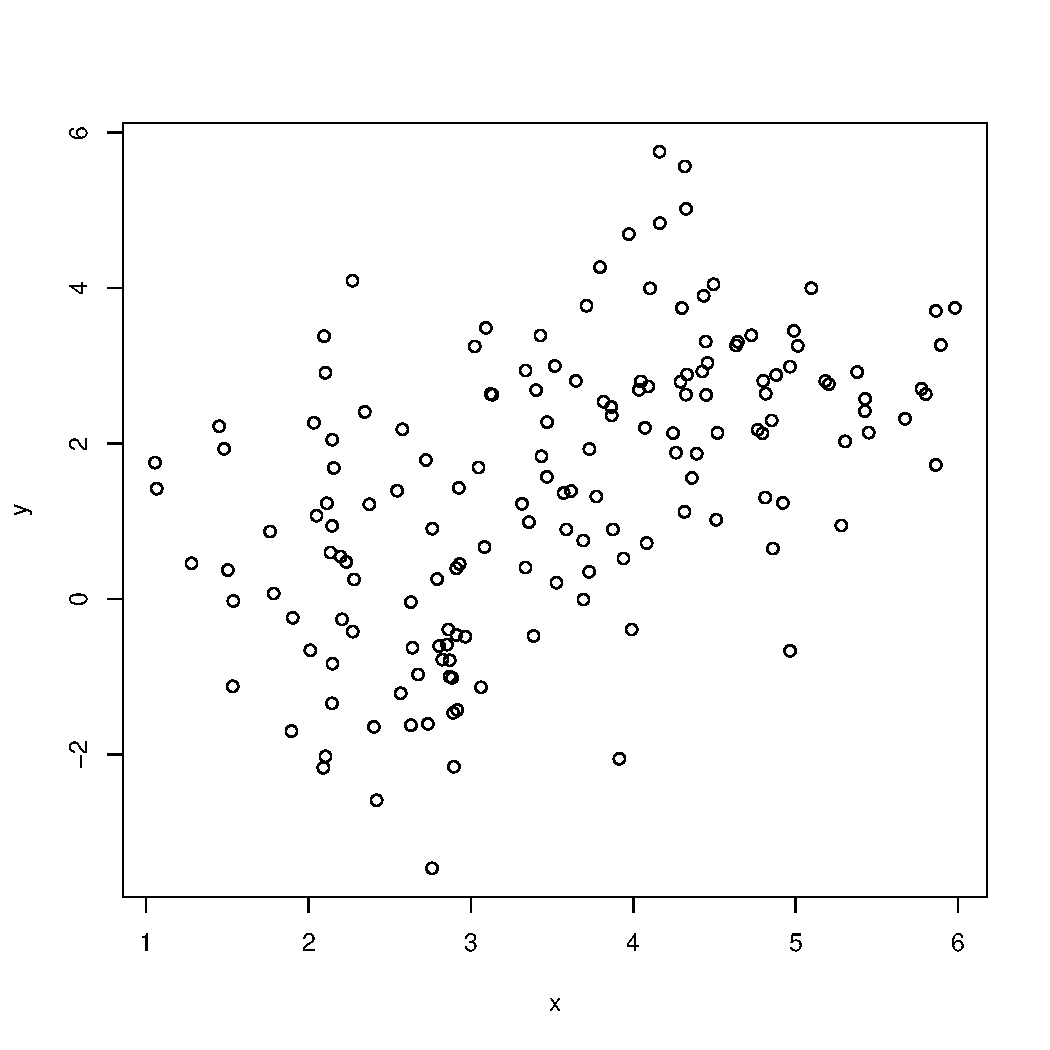
\includegraphics[width=\maxwidth]{figure/probability-Simpson-1} 

}

\caption[Scatter plot for the whole data]{Scatter plot for the whole data}\label{fig:probability-Simpson}
\end{figure}

\end{knitrout}

\begin{knitrout}
\definecolor{shadecolor}{rgb}{0.969, 0.969, 0.969}\color{fgcolor}\begin{kframe}
\begin{alltt}
\hlkwd{plot}\hlstd{(x, y,} \hlkwc{pch}\hlstd{=}\hlkwd{rep}\hlstd{(}\hlnum{1}\hlopt{:}\hlstd{g,} \hlkwc{each}\hlstd{=n),} \hlkwc{col}\hlstd{=}\hlkwd{rep}\hlstd{(}\hlnum{1}\hlopt{:}\hlstd{g,} \hlkwc{each}\hlstd{=n))}
\end{alltt}
\end{kframe}\begin{figure}

{\centering 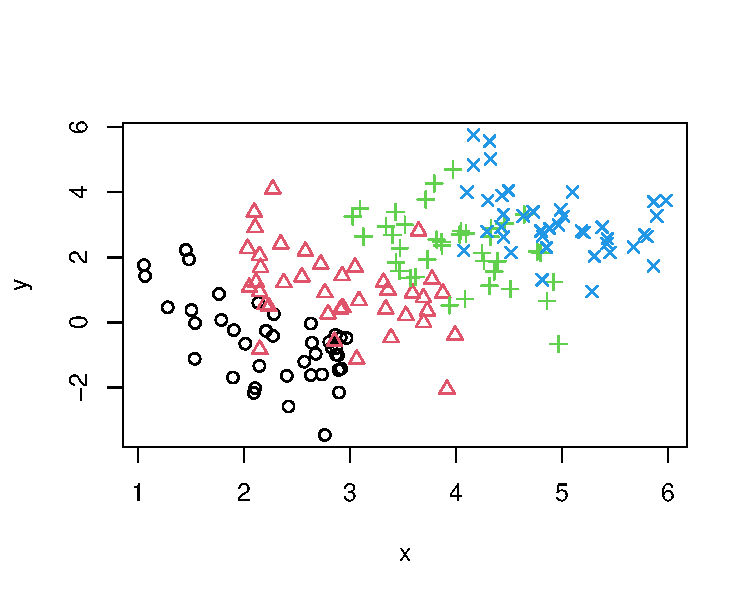
\includegraphics[width=\maxwidth]{figure/probability-Simpson2-1} 

}

\caption[Scatter plot with different groups labeled]{Scatter plot with different groups labeled}\label{fig:probability-Simpson2}
\end{figure}

\begin{kframe}\begin{alltt}
\hlcom{# label the points for different groups}
\end{alltt}
\end{kframe}
\end{knitrout}


We see that for the whole data, $y$ has an increase pattern as $x$
increases, but for each sub group $y$ has a decrease pattern as $x$
increases.

\hypertarget{prisoners-problem}{%
\section{100 prisoners problem}\label{prisoners-problem}}

The probability may help to obtain some changes in a seemingly
hopeless situation. Consider the following example modified from
\cite{flajolet2009analytic}.

In a prison, there are 100 death row prisoners who are numbered from 1
to 100, and there is a room with 100 drawers labeled from 1 to
100. The director randomly puts one prisoner's number in each closed
drawer and offers a last chance. The prisoners enter the room, one
after another. Each prisoner may open and look into 50 drawers in any
order. The drawers are closed again afterwards. If, during this
search, every prisoner finds his number in one of the drawers, all
prisoners are pardoned. If some prisoner does not find his number, all
prisoners die. Before the first prisoner enters the room, the
prisoners may discuss strategy, but they cannot communicate once the
first prisoner enters the room.

The situation is hopeless if every prisoner selects 50 drawers at
random. The probability that a single prisoner finds his number is
0.5, so the probability that all prisoners find their numbers is
$0.5^{100} = 7.89\times10^{31}\approx0$. However, a better strategy
gives the prisoners more than 0.30 probability to survive
\citep{stanley2013algebraic}. The strategy is described below.

\begin{enumerate}
\item Each prisoner first opens the drawer with his own number.
\item If this drawer contains his number he is done and was
  successful.
\item Otherwise, the drawer contains the number of another prisoner
  and he next opens the drawer with this number.
\item The prisoner repeats steps 2 and 3 until he finds his own number
  or has opened 50 drawers.
\end{enumerate}

In the following, we define two functions to simulate the method of randomly
open 50 drawers and the better strategy, respectively.

\begin{knitrout}
\definecolor{shadecolor}{rgb}{0.969, 0.969, 0.969}\color{fgcolor}\begin{kframe}
\begin{alltt}
\hlkwd{set.seed}\hlstd{(}\hlnum{2021}\hlstd{)}
\hlstd{n} \hlkwb{<-} \hlnum{100} \hlcom{# number of prisoners}
\hlstd{prisoners} \hlkwb{<-} \hlnum{1}\hlopt{:}\hlstd{n} \hlcom{# prisoners' numbers}
\hlcom{# simulate the procedure of randomly open 50 (n/2) drawers}
\hlstd{open.random} \hlkwb{<-} \hlkwa{function}\hlstd{(}\hlkwc{prisoners}\hlstd{,} \hlkwc{n}\hlstd{=}\hlkwd{length}\hlstd{(prisoners)) \{}
    \hlstd{drawers} \hlkwb{<-} \hlkwd{sample}\hlstd{(}\hlnum{1}\hlopt{:}\hlstd{n,} \hlkwc{size}\hlstd{=n,} \hlkwc{replace}\hlstd{=}\hlnum{FALSE}\hlstd{)}
    \hlcom{# randomly put prisoners’ numbers in the drawers}
    \hlstd{pardon} \hlkwb{<-} \hlnum{TRUE} \hlcom{# initialize pardon to be true}
    \hlkwa{for} \hlstd{(i} \hlkwa{in} \hlstd{prisoners) \{}
        \hlstd{opens} \hlkwb{<-} \hlkwd{sample}\hlstd{(drawers, n}\hlopt{/}\hlnum{2}\hlstd{)}
        \hlcom{# randomly open n/2 drawers}
        \hlkwa{if} \hlstd{(}\hlopt{!}\hlstd{(i} \hlopt \hlstd{opens)) \{}
            \hlcom{# if any prisoner does not find his number}
            \hlcom{# all prisoners die}
            \hlstd{pardon} \hlkwb{<-} \hlnum{FALSE}
            \hlkwa{break}
        \hlstd{\}}
    \hlstd{\}}
    \hlkwd{return} \hlstd{(pardon)}
\hlstd{\}}

\hlstd{open.smart} \hlkwb{<-} \hlkwa{function}\hlstd{(}\hlkwc{prisoners}\hlstd{,} \hlkwc{n}\hlstd{=}\hlkwd{length}\hlstd{(prisoners)) \{}
    \hlstd{drawers} \hlkwb{<-} \hlkwd{sample}\hlstd{(}\hlnum{1}\hlopt{:}\hlstd{n,} \hlkwc{size}\hlstd{=n,} \hlkwc{replace}\hlstd{=}\hlnum{FALSE}\hlstd{)}
    \hlstd{pardon} \hlkwb{<-} \hlnum{TRUE}
    \hlkwa{for} \hlstd{(i} \hlkwa{in} \hlstd{prisoners) \{}
        \hlstd{opens} \hlkwb{<-} \hlkwd{rep}\hlstd{(}\hlnum{NA}\hlstd{, n}\hlopt{/}\hlnum{2}\hlstd{)}
        \hlstd{opens[}\hlnum{1}\hlstd{]} \hlkwb{<-} \hlstd{drawers[i]}
        \hlkwa{for} \hlstd{(j} \hlkwa{in} \hlnum{2}\hlopt{:}\hlstd{(n}\hlopt{/}\hlnum{2}\hlstd{))\{}
            \hlkwa{if} \hlstd{(opens[j}\hlopt{-}\hlnum{1}\hlstd{]} \hlopt{==} \hlstd{i) \{}
                \hlkwa{break}
            \hlstd{\}} \hlkwa{else} \hlstd{\{}
                \hlstd{opens[j]} \hlkwb{<-} \hlstd{drawers[opens[j}\hlopt{-}\hlnum{1}\hlstd{]]}
            \hlstd{\}}
        \hlstd{\}}
        \hlkwa{if} \hlstd{(}\hlopt{!}\hlstd{(i} \hlopt \hlstd{opens)) \{}
            \hlstd{pardon} \hlkwb{<-} \hlnum{FALSE}
            \hlkwa{break}
        \hlstd{\}}
    \hlstd{\}}
    \hlkwd{return} \hlstd{(pardon)}
\hlstd{\}}
\hlcom{# survival probability of randomly open}
\hlkwd{mean}\hlstd{(}\hlkwd{replicate}\hlstd{(}\hlnum{10000}\hlstd{,} \hlkwd{open.random}\hlstd{(prisoners)))}
\end{alltt}
\begin{verbatim}
## [1] 0
\end{verbatim}
\begin{alltt}
\hlcom{# survival probability of using the better strategy}
\hlkwd{mean}\hlstd{(}\hlkwd{replicate}\hlstd{(}\hlnum{10000}\hlstd{,} \hlkwd{open.smart}\hlstd{(prisoners)))}
\end{alltt}
\begin{verbatim}
## [1] 0.2999
\end{verbatim}
\end{kframe}
\end{knitrout}


\hypertarget{Monty-Hall-problem}{%
\section{Monty Hall problem}\label{Monty-Hall-problem}}

% The problem was originally posed (and solved) in a letter by Steve Selvin to
% the American Statistician in 1975.  Selvin, Steve (February 1975a). "A problem
% in probability (letter to the editor)". The American Statistician. 29 (1):
% 67–71.  Selvin, Steve (February 1975a). "A problem in probability (letter to
% the editor)". The American Statistician. 29 (1): 67–71.  It became famous as a
% question from reader Craig F. Whitaker's letter quoted in Marilyn vos Savant's
% "Ask Marilyn" column in Parade magazine in 1990: Selvin, Steve (February
% 1975a). "A problem in probability (letter to the editor)". The American
% Statistician. 29 (1): 67–71.  The Monty Hall problem is mathematically
% equivalent to the earlier Three Prisoners problem Gardner, Martin (October
% 1959). "Mathematical Games: Problems involving questions of probability and
% ambiguity". Scientific American. 201 (4): 174–182.  Gardner, Martin
% (1959). "Mathematical Games: How three modern mathematicians disproved a
% celebrated conjecture of Leonhard Euler". Scientific American. 201 (5): 188

Suppose you're on a game show, and you're given the choice of three doors:
Behind one door is a car; behind the others, goats. You pick a door, say No. 1,
and the host, who knows what's behind the doors, opens another door, say No. 3,
which has a goat. He then says to you, "Do you want to pick door No. 2?" Is it
to your advantage to switch your choice?

\begin{knitrout}
\definecolor{shadecolor}{rgb}{0.969, 0.969, 0.969}\color{fgcolor}\begin{kframe}
\begin{alltt}
\hlkwd{set.seed}\hlstd{(}\hlnum{2021}\hlstd{)}
\hlstd{n} \hlkwb{<-} \hlnum{1000}
\hlstd{first} \hlkwb{<-} \hlnum{1}
\hlstd{prize} \hlkwb{<-} \hlkwd{rep}\hlstd{(}\hlnum{NA}\hlstd{, n)}
\hlstd{host} \hlkwb{<-} \hlkwd{rep}\hlstd{(}\hlnum{NA}\hlstd{, n)}
\hlkwa{for} \hlstd{(i} \hlkwa{in} \hlnum{1}\hlopt{:}\hlstd{n)\{}
    \hlstd{prize[i]} \hlkwb{<-} \hlkwd{sample}\hlstd{(}\hlnum{1}\hlopt{:}\hlnum{3}\hlstd{,} \hlnum{1}\hlstd{)}
    \hlkwa{if} \hlstd{(prize[i]} \hlopt{==} \hlnum{1}\hlstd{)\{}
        \hlstd{host[i]} \hlkwb{<-} \hlkwd{sample}\hlstd{(}\hlkwd{c}\hlstd{(}\hlnum{2}\hlstd{,} \hlnum{3}\hlstd{),} \hlnum{1}\hlstd{)}
    \hlstd{\}} \hlkwa{else if} \hlstd{(prize[i]} \hlopt{==} \hlnum{2}\hlstd{) \{}
        \hlstd{host[i]} \hlkwb{<-} \hlnum{3}
    \hlstd{\}} \hlkwa{else if} \hlstd{(prize[i]} \hlopt{==} \hlnum{3}\hlstd{) \{}
        \hlstd{host[i]} \hlkwb{<-} \hlnum{2}
    \hlstd{\}}
\hlstd{\}}
\hlstd{observed} \hlkwb{<-} \hlstd{prize[host} \hlopt{==} \hlnum{3}\hlstd{]}
\hlkwd{sum}\hlstd{(observed} \hlopt{==} \hlnum{2}\hlstd{)} \hlopt{/} \hlkwd{length}\hlstd{(observed)}
\end{alltt}
\begin{verbatim}
## [1] 0.6707566
\end{verbatim}
\end{kframe}
\end{knitrout}



%%% Local Variables:
%%% coding: utf-8
%%% mode: latex
%%% TeX-master: "00why.tex"
%%% End:

%%% TeX-engine: xetex
%%% TeX-command-extra-options: "-shell-escape"


\hypertarget{ch:estimation}{%
\chapter{Estimation: A hide-and-seek game with the nature}\label{ch:estimation}}


\section{Introduction}
Consider this game setup. We have a random sample of size \(n\) from a normal
distribution \(N(\mu, 1)\), where \(\mu\) is unknown, and we want to estimate \(\mu\)
with this sample. An estimator is a quantity constructed from the observed
sample, that is, it is a statistic. What estimators can we construct? How do we
assess which is better?

\input{Rnw/est-hide-normal}

\section{Seeking strategies}

To play the hide-and-seek game better, we need to select a good strategy. From
the examples in the last section, it seems that which strategy is better depends
on the underlying truth, which is unknown.


Let's start with an example.
\begin{illustration}[Likelihood in guessing jars]
  % \indexExSix{Computing ranks in the presence of ties}
\label{example:has-jars}
There are 9 jars. The first jar has 9 red and 1 green balls; the second jar has
8 red and 2 green balls; $\cdots\cdots$; the 9th jar has 1 red and 9 green
balls. Now, one jar is randomly selected, from which one ball is randomly
selected, and the ball is red. Which jar was the one that was selected?

There are nine possibilities. If the selected jar were the first one, the
probability that a randomly selected ball is red is 9/10. If the selected jar
were the second one, the probability that a randomly selected ball is red is
8/10. Continue until the 9th jar. With this calculation, which jar should we
guess?

The first one!
\end{illustration}

The principle we use here is the so-called maximum likelihood estimation. The
unknown true has 9 possibilities. We choose the one that gives the highest
likelihood of observing a randomly selected ball being red.


% The area of a circle with radiur \(r\) is

% \begin{align}
%     R = \pi r^2.
% \label{eq:area}
% \end{align}

% \begin{align*}
% \mathrm{MSE}(\hat\mu) = (\hat\mu - \mu)^2
% \end{align*}



\hypertarget{ch:hypothesis}{%
\chapter{Hypothesis testing}\label{ch:hypothesis}}

Hypothesis testing can be thought of as a stochastic analog of proof by
contradiction.

``To understand the essence of statistical hypothesis testing properly, it is
necessary to compare intentionally hypothesis testing with proof by
contradiction and characterize the former as not the same as the latter.''
\citep{otani2019comparing}.

It should be relatively clear, then, why a failure to reject H , does not
constitute a verification of its truth. It simply means that the researcher has
failed to provide evidence suflcient to cast serious doubt on the truth of
\(H_0\). \citep{reeves1980hypothesis}

Misconception \citep{falk1995significance}.


\bibliography{book.bib,packages.bib}

\backmatter

\printindex

\end{document}
